\chapter{Reproduktion bisheriger Ergebnisse}
\label{chap:reproduktion}
\epigraph{What I cannot create, I do not understand}{--- Richarch Feyman}

\qq{Warum NN?}
Künstliche Neuronale Netzwerke (kurz NN) dominieren den Forschungsbereich der 
Bilderkennung dank vieler Erfolge. 
Besonders die Klasse der faltenden Neuronalen Netzwerks (engl. Convolutional Neural Network, kurz CNN) konnte viele Erfolge für sich beanspruchen.
Rekordbrechende Erfolge bei der Klassifiziererung von handgeschriebenen Ziffern \parencite{LeCunBackpropagationappliedhandwritten1989} und des ImageNet-Wettbewerbs \parencite{KrizhevskyImageNetClassificationDeep2012a} motivieren dazu CNN-Methoden auch in anderen
Bereichen anzuwenden.

Neurale Netzwerke benötigen weniger Entwicklungsaufwand und können zudem einfacher von der 
von wachsenden Resourzen und Datenmengen gebrauch machen \parencite[436]{LeCunDeeplearning2015}. 
Aber die Wissenschaft der NN ist ein Feld, dass durch die aktuelle Praxis mehr als durch Theorie geprägt ist. Das beudeuted zum einen das theoretische Grundlagen noch nicht gefestigt sind.
Zum anderen ist die Theorie nur eine Faktor für den erfolgreichen Einsatz von NNs. 

Je mehr Parameter unklar sind desto schwieriger wird eine Reproduktion.
Im folgenden werden Paper genauer untersucht, die sich mit dem Problem der Dokumentensegmentierung mit Hilfe von 

Die Reproduktion ist ein wichtiger Bestandteil in jedem Forschungsgebiet. 


Das erste Experiment basiert auf dem neusten Paper von Mitgliedern der DIVA-Gruppe: \citeauthor*{ChenConvolutionalNeuralNetworks2017}. 
\qq{welche Experimente?}
Das zweite Experiment basiert auf der Forschung des Gewinners des IDCAR2017-Wettbewerbs: \citeauthor*{XuPageSegmentationHistorical2017} 

\section{Bildverarbeitung mittels Neuronaler Netzwerke}
Einleitung \cite{LeCunDeeplearning2015}

\section{SGD}
\section{Aktivierungsfunktionen}
\subsection{ReLU}
\begin{align}
    f\left(x\right) &= \text{max}(0,x)
\end{align}
\subsection{Softmax}


\section{CNN}
\qq{Filter als vorläufer von CNN}
CNN kombinieren zwei Konzepte der Bilderverarbeitung: Neuronale Netzwerke und Filter.
Klassifikationsprobleme wurde traditionell in zwei Schritten gelöst. Zuerst wurden 
Featuredeskriptoren entwickelt welche dann als Input für trainierbare Klassifizierer 
verwendet wurden \autocite[2353]{RawatDeepConvolutionalNeural2017}.

\qq{Filterbeispiel?}
\qq{}

\section{\textcite{ChenConvolutionalNeuralNetworks2017}}
Das Paper ``\citetitle*{ChenConvolutionalNeuralNetworks2017}'' von \citeauthor*{ChenConvolutionalNeuralNetworks2017} betrachten die Dokumentensegmentierung 
als ``pixel labeling problem''. Einem Pixel wird eine Klasse zugewiesen indem
ein CNN die Umgebung des Pixels analisiert. 
Jedoch ist eines der größten Probleme bei der Verarbeitung von Dokumentenseiten die Größe.
Die Bilder im HisDB-Datenset sind mit einer Auflösung von \(4872 \times 6496\) wesentlich größer als andere Datensets.\qq{Welche?}
Um den Prozess zu beschleunigen werden nicht alle Pixel sondern nur etwa 3000 Pixelcluster klassifiziert. 

\subsection{Vorverarbeitung}
\citeauthor{ChenConvolutionalNeuralNetworks2017} skalieren alle Bilder mit einem Faktor von  \(2^{-3}\) und wenden dann den Superpixelalgorithmus SLIC (simple linerar iterative clustering) an \parencite{AchantaSLICSuperpixels2010} um die Dokumentenseiten in Superpixel einzuteilen.
Ein \(28 \times 28\)-Bereich um das Zentrum des Superpixel wird dann mithilfe eines CNN
klassifiziert. Diese Klassifizierung wird dann allen Pixel innerhalb des Superpixels zugewiesen.

\section{SLIC Superpixel}
Der SLIC-Algorithmus basiert auf dem k-Means-Algorithmus und teilt Pixel inhalb eines 5D-Raums in Cluster ein. 
In jedem Arbeitsschritt werden Pixel dem Clusterzentrum mit der geringsten Distanz zugeordnet und danach werden die Clusterzentren neu berechnet.
Das Distanzmaß \(D_s\) zu den Clusterzentren \(k=[1,K]\) basiert auf den Farbabstand im Lab-Farbraum \(d_{lab}\) und den räumlichen Abstand \(d_{xy}\):

\begin{align}
    d_{lab} &= \sqrt{ \left( l_k - l_i \right)^2 + \left( a_k - a_i \right)^2 + \left( b_k - b_i \right)^2 }\\
    d_{xy}  &= \sqrt{ \left( x_k - x_i \right)^2 + \left(y_k - y_i \right)^2 }\\
    D_{s}   &= d_{lab} + \frac{m}{S} d_{xy}
\end{align}

Der Faktor \(m\) ermöglicht eine Gewichtung den zwei Distanzmaßen. Je höher
der Faktor desto kompakter werden die Superpixel. \cref{fig:slic_parameters}
zeigt das Ergebniss des Algorithmus mit unterschiedlichen Parameter  \(m\)
angewendet auf eine Dokumentenseite.

\begin{figure}
    \centering
    \caption{Die SLIC-Pixelgrenzen sind in rot dargestellt }
    \label{fig:slic_parameters}
    \subfloat[ \(m = 0.1\)]{
        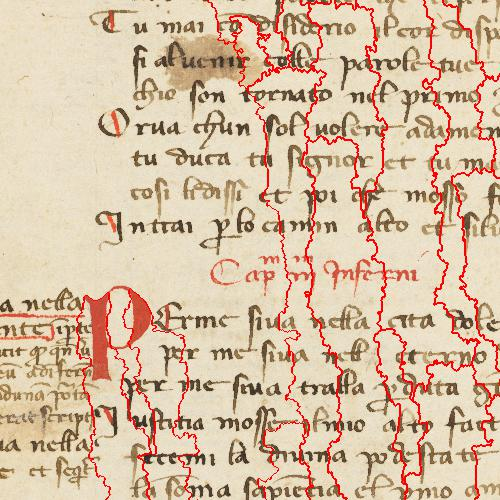
\includegraphics[width=0.24\textwidth]{figures/img/mark_boundaries_m0.jpg}
    }
    \subfloat[\(m = 1\)]{
        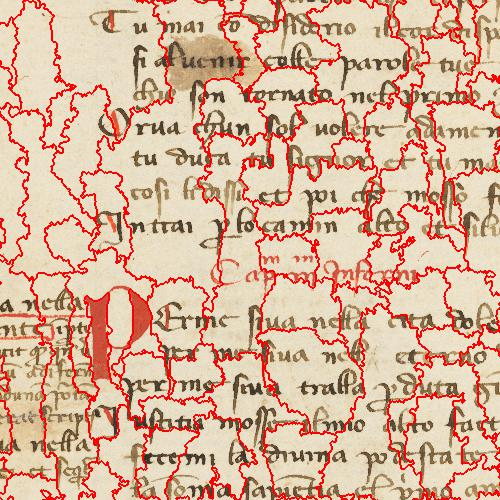
\includegraphics[width=0.24\textwidth]{figures/img/mark_boundaries_m1.jpg}
    }
    \subfloat[\(m = 10\)]{
        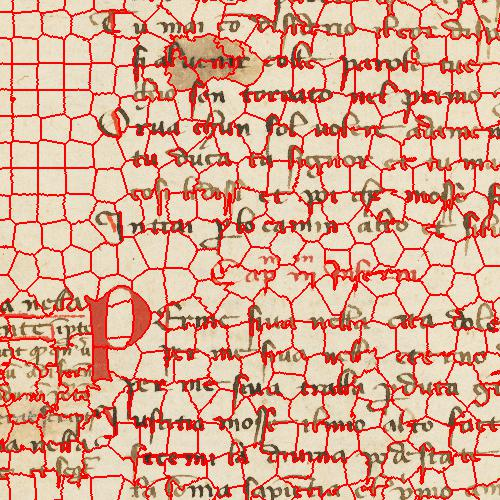
\includegraphics[width=0.24\textwidth]{figures/img/mark_boundaries_m10.jpg}
    }
    \subfloat[\(m = 100\)]{
        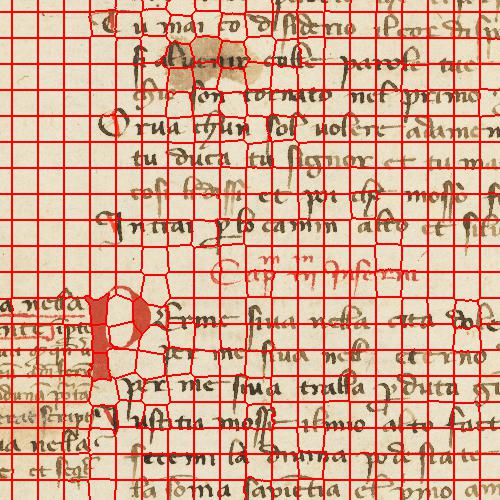
\includegraphics[width=0.24\textwidth]{figures/img/mark_boundaries_m100.jpg}
    }
\end{figure}

\citeauthor{AchantaSLICSuperpixelsCompared2012} stellen später zwei wichtige Erweiterungen vor:
Normalisierung des Distanzmaßes und Adaptive-SLIC.

\citeauthor{ChenConvolutionalNeuralNetworks2017a} nennen keine Details zur Wahl
der Superpixel-Parameter.

\section{CNN-Architektur}
\citeauthor{ChenConvolutionalNeuralNetworks2017a} beschreiben die Struktur
des CNN als \(28 \times 28 \times 1 - 26 \times 26 \times 4 - 100 - M\).

Während des Trainings wird das Ground-truth Label des Zentrumpixels als Label für den Superpixel verwendet.


\section{Xavier initialization}


\section{Dropout}

\subsection{PyTorch}
% Genauer klären
PyTorch ist ein Framework zur automatischen Differenzierung von skaler Funktion \autocite{PaszkeAutomaticdifferentiationPyTorch2017}.

\section{Training}


\section{\textcite{XuPageSegmentationHistorical2017}}
Das Paper ``\citetitle*{XuPageSegmentationHistorical2017}'' von \citeauthor*{XuPageSegmentationHistorical2017}.

\section{VGG}
\section{Deconvolution}
\section{Ergebnisse}